\documentclass[11pt,a4paper,DIV=10,]{scrartcl}
\usepackage[utf8]{inputenc}
\usepackage[ngerman]{babel}
\usepackage{amsmath}
\usepackage{amsfonts}
\usepackage{amssymb}
\usepackage{amsthm}
\usepackage{fancybox}
\usepackage{multicol}
\usepackage{graphicx}
\usepackage{float}
\usepackage{listings}
\usepackage{color}
\usepackage{colortbl}

% Define user colors using the RGB model
\definecolor{dunkelgrau}{rgb}{0.8,0.8,0.8}
\definecolor{hellgrau}{rgb}{0.95,0.95,0.95}
\definecolor{middlegray}{rgb}{0.5,0.5,0.5}
\definecolor{lightgray}{rgb}{0.8,0.8,0.8}
\definecolor{orange}{rgb}{0.8,0.3,0.3}
\definecolor{yac}{rgb}{0.6,0.6,0.1}

% Zitation und Literaturverzeichnis
\usepackage[normal,font={small,color=black}, labelfont=bf,figurename=Abb.]{caption}
\usepackage{cite}
\usepackage{url}
\bibliographystyle{unsrtnat}
\usepackage[numbers]{natbib}
%\usepackage[T1]{fontenc}

\begin{document}
% Formatierung für das Listing
\lstset{
   basicstyle=\scriptsize\ttfamily,
   keywordstyle=\bfseries\ttfamily\color{orange},
   stringstyle=\color{green}\ttfamily,
   commentstyle=\color{middlegray}\ttfamily,
   emph={square}, 
   emphstyle=\color{blue}\texttt,
   emph={[2]root,base},
   emphstyle={[2]\color{yac}\texttt},
   showstringspaces=false,
   flexiblecolumns=false,
   tabsize=2,
   numbers=left,
   numberstyle=\tiny,
   numberblanklines=true,
   stepnumber=1,
   numbersep=10pt,
   xleftmargin=15pt
}

\subsection*{DBS SoSe 2013, Di. 8-10}
\section*{Projektdokumentation: Iteratation No. 3}
\textbf{Christoph van Heteren-Frese (Matr.-Nr.: 4465677), \\ Sven Wildermann (Matr.-Nr.: 4567553) }
\hrule
\section{Rahmenbedingungen}
\begin{enumerate}
\item[•] DBS: PostgreSQL
\item[•]JavaServer Pages (JSP): Apache Tomcat 7
\end{enumerate}
\section{Modellierung}
Wir modellieren unser Datenbankschema wie folgt: \\
Da wir davon ausgehen, dass nicht regelmäßig neue Wetterstationen entstehen oder abgebaut werden, haben wir die Relation ``hat kürzeste Distanz zu'' gebildet. Diese muss aktualisiert werden, sobald sich die Wetterstationen ändern. Wenn eine neue Stadt (bzw. ``location'') hinzu kommt oder entfernt wird, reicht es entsprechend einen Eintrag hinzuzufügen bzw. zu entfernen. \\
Da die Wetterdaten über einen Schlüssel eindeutig mit den Wetterstationen verknüpft sind, haben wir hier eine Relation ``führt durch''. Im Endeffekt wird hier jede Verknüpfung zwischen einer Wettermessung und einem Standort hergestellt. Aktualisieren sich die Wettermessungen, so muss auch diese Relation aktualisiert werden. \\
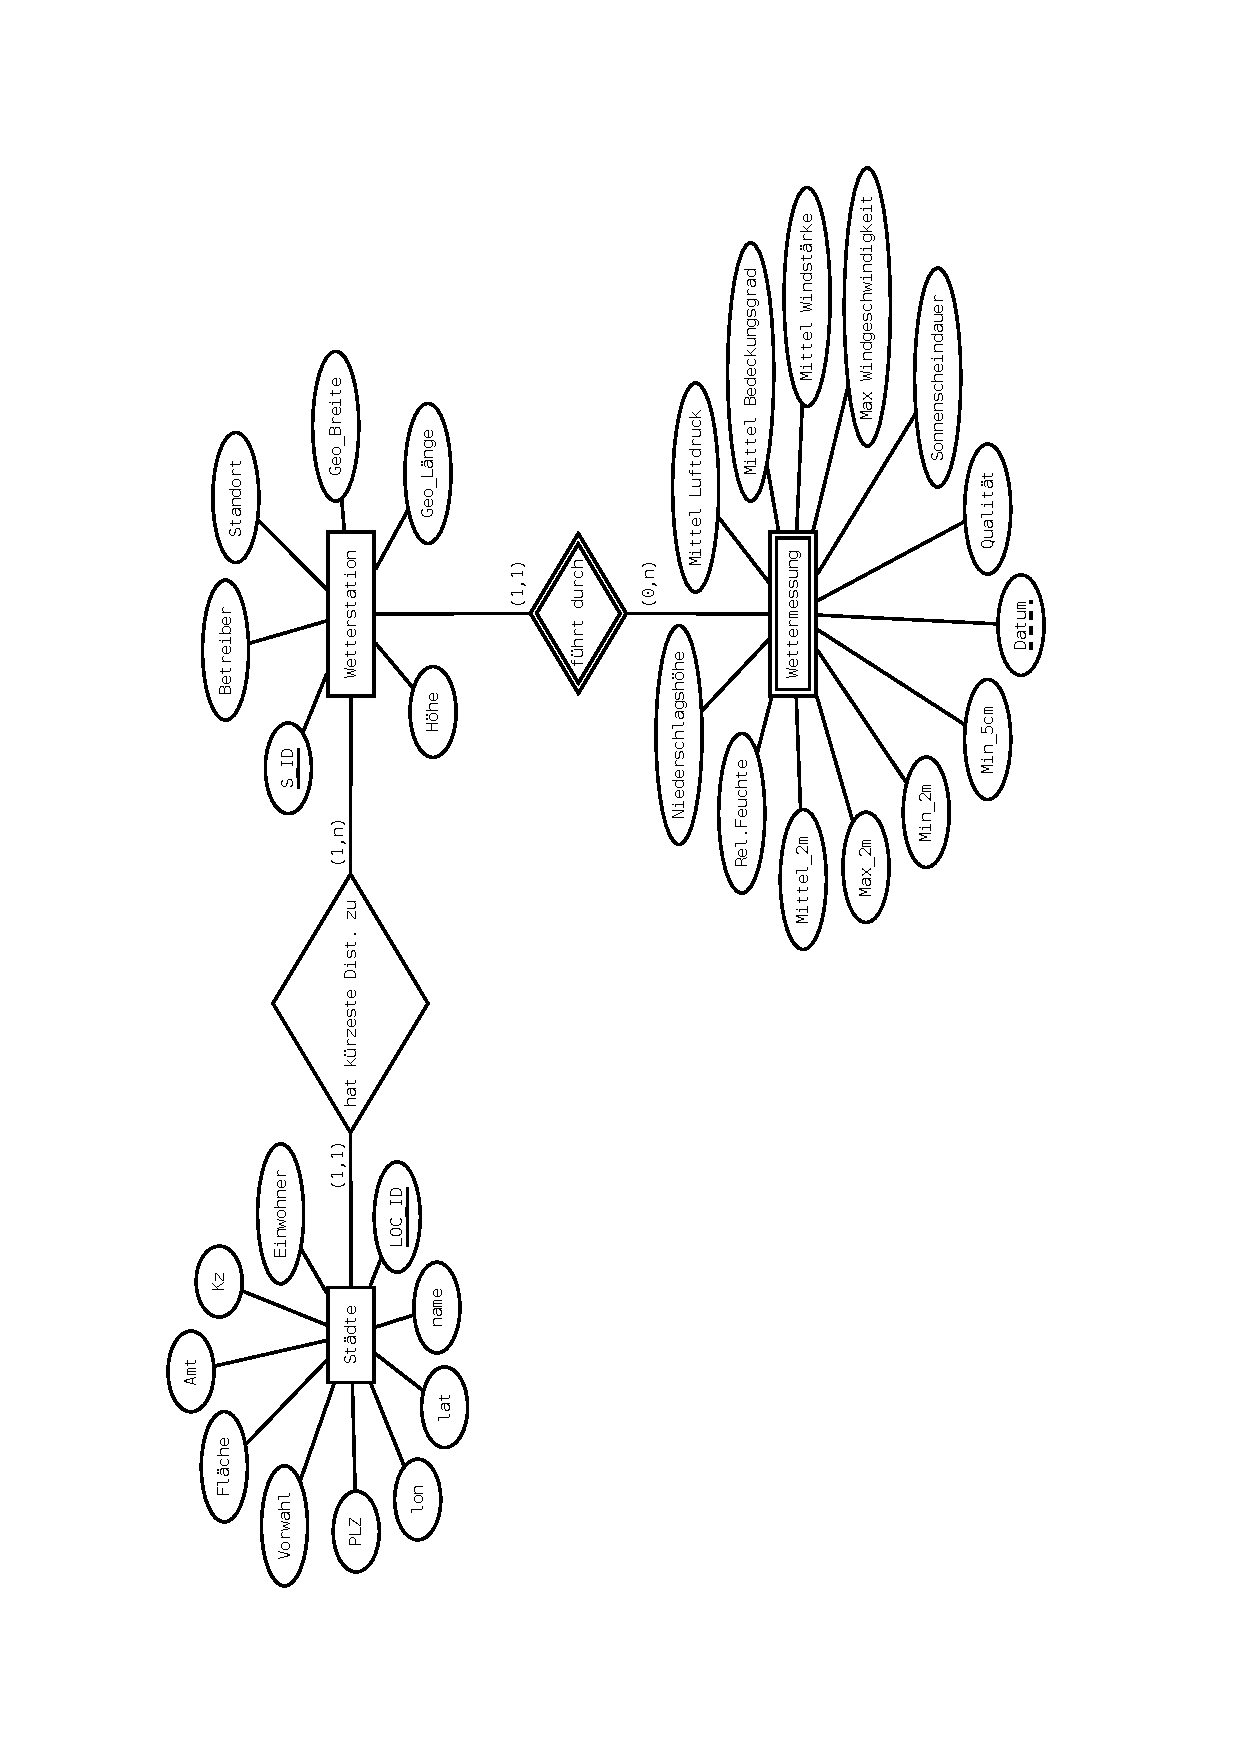
\includegraphics[width=13cm, angle=270]{Diagram1.pdf}
\section{Herkunft der Daten}
Die Daten der Städte stammen aus der frei zugänglichen Datenbank GeoDB. Die Wetterdaten werden von der Uni Bayreuth zur Verfügung gestellt. 
\section{Erzeugen der Relationen/Tabellen}
Die erzeugten Relationen weichen teilweise von den in \citep{geodb.org} dokumentierten Schemata ab. 
\subsection*{Beispiel: geodb\_intdata}
\begin{lstlisting}[language=sql]
CREATE TABLE geodb_intdata (
    loc_id integer,
    int_type integer,
    int_val integer,
    valid_since date,
    date_type_since integer,
    valid_until date,
    date_type_until integer
);
\end{lstlisting}
\subsection*{Beispiel: staedte}
\begin{lstlisting}[language=sql]
CREATE TABLE staedte (
	id serial NOT NULL PRIMARY KEY,
	plz VARCHAR ( 10 ) NOT NULL ,
	name VARCHAR ( 255 ) NOT NULL ,
	vorwahl text,	
	einwohner integer,
	flaeche float,
	amt text, 
	kz varchar (3),
	lat float,
	lon float
);
\end{lstlisting}
\section{Datenimport}
Zeilen, die der JOIN-Bedingung nicht genügen, werden durch 'OUTER LEFT JOIN' nur dann in die Zieltabelle eingefügt, wenn keine weiteren Bedingungen dies verhindern. Letzteres ist genau  genau dann der Fall, wenn der gewünschte Texttyp im WHERE-Statement 'selektiert' wird. Daher muss dies bereits in der Joinbedingung geschehen.
\subsection*{Beispiel: Städte-Relation}
\begin{lstlisting}[language=sql]
INSERT INTO staedte (plz, name, vorwahl, einwohner, flaeche, amt, kz, lat, lon)
	SELECT plz.text_val1 as plz, name.text_val1 as name, vorwahl.text_val1 as vorwahl,
		einw.int_val as einwohner, flaeche.float_val as flaeche, amt.text_val1 as amt,
		kz.text_val1 as kz, coord.lat,coord.lon
	FROM geodb_textdata plz
	LEFT OUTER JOIN geodb_textdata name 
		ON plz.loc_id = name.loc_id
	LEFT OUTER JOIN geodb_textdata vorwahl 
		ON (plz.loc_id = vorwahl.loc_id AND vorwahl.text_type = 500400000)
	LEFT OUTER JOIN geodb_floatdata flaeche 
		ON (plz.loc_id = flaeche.loc_id AND flaeche.float_type = 610000000)
	LEFT OUTER JOIN geodb_intdata einw 
		ON (plz.loc_id = einw.loc_id AND einw.int_type = 600700000)
	LEFT OUTER JOIN geodb_textdata amt 
		ON (plz.loc_id = amt.loc_id AND amt.text_type = 500700000)
	LEFT OUTER JOIN geodb_textdata kz 
		ON (plz.loc_id = kz.loc_id AND kz.text_type = 500500000)
	LEFT OUTER JOIN geodb_locations gl 
		ON (plz.loc_id = gl.loc_id AND gl.loc_type IN (100600000 ,100700000))
	LEFT OUTER JOIN geodb_coordinates coord 
		ON plz.loc_id = coord.loc_id
	WHERE plz.text_type = 500300000
		AND name.text_type = 500100000 ORDER by name, plz;
\end{lstlisting}

\section{Berechnung der Relation ``hat kürzeste Distanz zu''}
Für die Berechnung der Relation ``hat kürzteste Distanz zu'', die zwischen den Städten und den Wetterstationen vorliegt, 
wurden eigene SQL-Funktionen implementiert.\\
Die erste Funktion berechnet den Abstand zwischen zwei Koordinaten in km auf einer Kugel, so dass nicht nur die Distanz innerhalb Deutschlands korrekt berchnet wird, sondern auch die Entfernungen zwischen zwei weiter von einander entfernten Punkten. 
\lstinputlisting[language=sql]{twopoints.sql}

Die zweite Funktion iteriert die Funktion distance auf allen Städten zu allen Wetterstationen, nimmt nur den kürzesten Eintrag einer Stadt zu einer Wetterstation und fügt diesen Eintrag in die Tabelle shortestdistance hinzu. Wenn diese Berechnung für alle Datensätze erneut durchgeführt werden muss, muss zuerst geprüft werden welchen Index der letzte Datensatz in der Relation städte hat (um diesen in der Funktion bei Abweichung zu ersetzen) und die Relation shortestdistance muss vorher geleert werden. 
\lstinputlisting[language=sql]{shortestdistance.sql}

\section{Web-Anwendung}

\bibliographystyle{agsm}
\bibliography{dbs}

\end{document}